\documentclass[twocolumn, amsmath]{revtex4}


\usepackage{graphicx}


\begin{document}


\title{PHYS 605 Lab \#1} 

\author{Evin O'Shea}  % fill in your name here
\email{eco2000@wildcats.unh.edu}  % add your email address 
\date{\today}  


\begin{abstract}
A voltage divider can allow an input voltage to be decreased to produce a lowered output voltage. In the lab, the group designed two voltage dividers, each to provide 2.7V output from a 5V input. In the first part of the lab, the goal was simply to create a cicuit that drove the voltmeter to measure the output voltage. In the second part, an actual load was attatched to the circuit and the output voltage along with the sag were measured. The group was successful in achieving the desired outpouts of 2.7V and minimizing the sag.
	

\end{abstract}

\maketitle

%
%  Now that the initial formatting and first-page details are set, let's add some relevant sections to the paper
%
\section{Background}

Part A of the lab asked the group to design a voltage divider that would provide 2.7V using a 5.00V input and a few k$\Omega$ resistors.

Part B of the lab asked the group to design a voltage divider that would also provide 2.7V output with a 5.00V input. This part of the lab also asked the group to add a load to the votage divider and to desgin the circuit so that when the load was added, the sag was less than 0.2V.
	


\section{Methodology}

For part A of the lab, the voltage divider had to output 2.7V. To do this, the group had to solve the equation governing the voltage divider circuit. This equation is shown below:

\begin{equation}
V_{out} = V_{in}\frac{R_2}{R_1 + R_2}
\end{equation}

This equation can be rearranged to calculate the ratio $\frac{R_1}{R_2}$ as shown below:

\begin{equation}
\frac{R_1}{R_2} = \frac{V_{in}}{V_{out}}-1
\end{equation}

The group plugged in the values $V_{in}$ = 5.00V and $V_{out}$ = 2.7V to equation (2) and got that $\frac{R_1}{R_2}$ = 0.852. The accessible resistors included 150k$\Omega$ and 130k$\Omega$. This ratio would be $\frac{R_1}{R_2} = \frac{130k\Omega}{150k\Omega} = 0.867$. The group then used equation (1) to calculate the output voltage $V_{out} = 5.00V\frac{150k\Omega}{130k\Omega + 150k\Omega} = 2.68V$. Furthermore, 2.679V would have a 0.7937\% error compared to 2.7V.


For part A of the lab, sag was not considered as the voltage divider only drove the voltmeter, which has a high resistance and would not cause signifigant sag. For part B of the lab, the circuit had to be designed to minimize sag. Sag occurs when a load is attatched to a voltage divider. When the load (denoted $R_L$) is attatched, the $R_2$ from equation (1) becomes $R_2'$ and follows the relation shown below:

\begin{equation}
R_2' = \frac{R_2R_L}{R_2 + R_L}
\end{equation}

However, in the limit that $R_L \gg R_2$, then $R_2' \approx R_2$. In order to reduce the sag, the group designed the voltage divider to use resistors several orders of magnitude smaller than the load. A 22.6$\Omega$ resistor and a 27$\Omega$ resistor were used for $R_1$ and $R_2$ respectively. Only using equation (1), this provide an output voltage $V_{out} = 5.00V\frac{27\Omega}{22.6\Omega + 27\Omega} = 2.72V$. In order to account for the load, the group used equation (3) to calculate $R_2'$. For $R_L$, the group used a 150k$\Omega$ resistor. $R_2' = \frac{27\Omega x150,000\Omega}{27\Omega + 150,000\Omega} = 26.995\Omega$. Then, the group calculated the expected output voltage using the value of $R_2'$ and equation (1). $V_{out}' = 5.00V\frac{26.995\Omega}{22.6\Omega + 26.995\Omega} = 2.7216V$. The sag in this case would be $V_{out} - V_{out}' \approx 0.0002$. This would be a very small sag and would meet the lab requirements.


\section{Results and Analysis}

For part A of the lab, the circuit constructed is shown below:

\begin{figure}[h]  
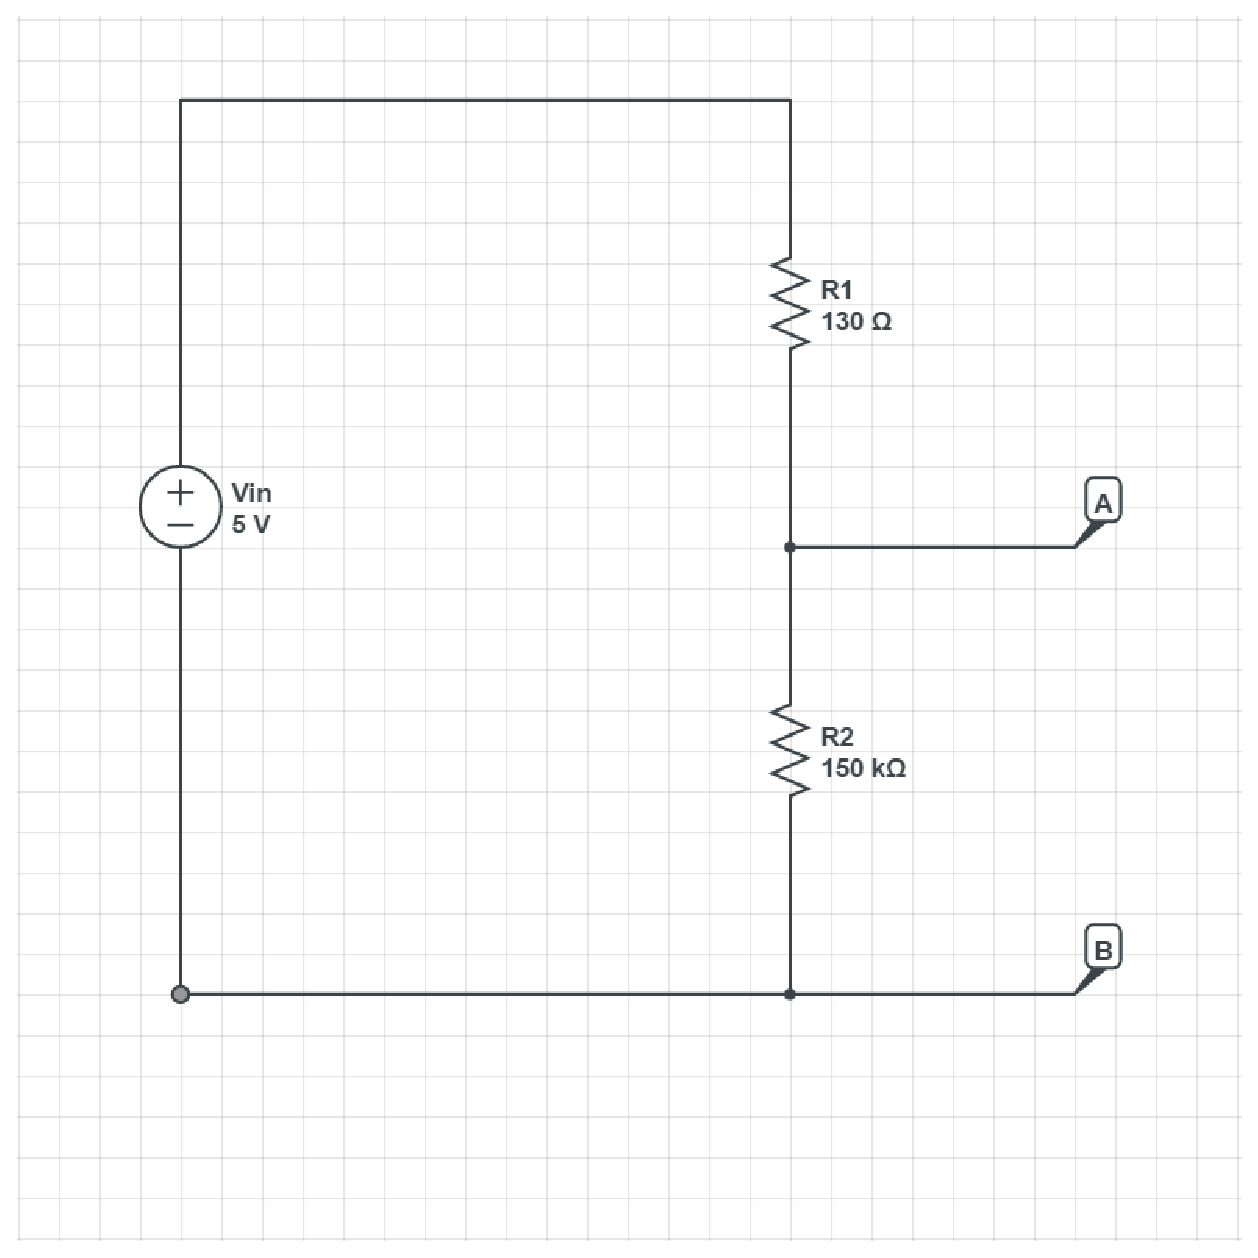
\includegraphics[scale = 0.3]{DIAGRAM1lab1.eps}  
\graphicspath{ {/home/evin/Desktop/School/Circuits/lab1/} }
\end{figure}

This circuit is designed to have a load connected to terminals A and B and is to produce an output voltage of 2.679V. The output voltage measured by the voltmeter was 2.689V. This gives a 0.4108\% error from the calculated value of 2.679V. The measured output voltage also had a 0.4074\% error from the goal of 2.7V. This design works well for the goal of the lab. The measured output was close to both the calculated output voltage and the goal output voltage. The design was successful in achieving an output voltage close to 2.7V. Though the values were close, the output voltage was higher than expected. This means that some part of the design was not perfect and could have been improved. The most likely cause of the inaccuracy was that the resistors used in the lab were not measured before use. This means that they may not have had the exact value that they were labeled as. This assumption by the lab group was the main cause of the error in the lab.

For part B of the lab, the circuit constructed is shown below:

\begin{figure}[h]  
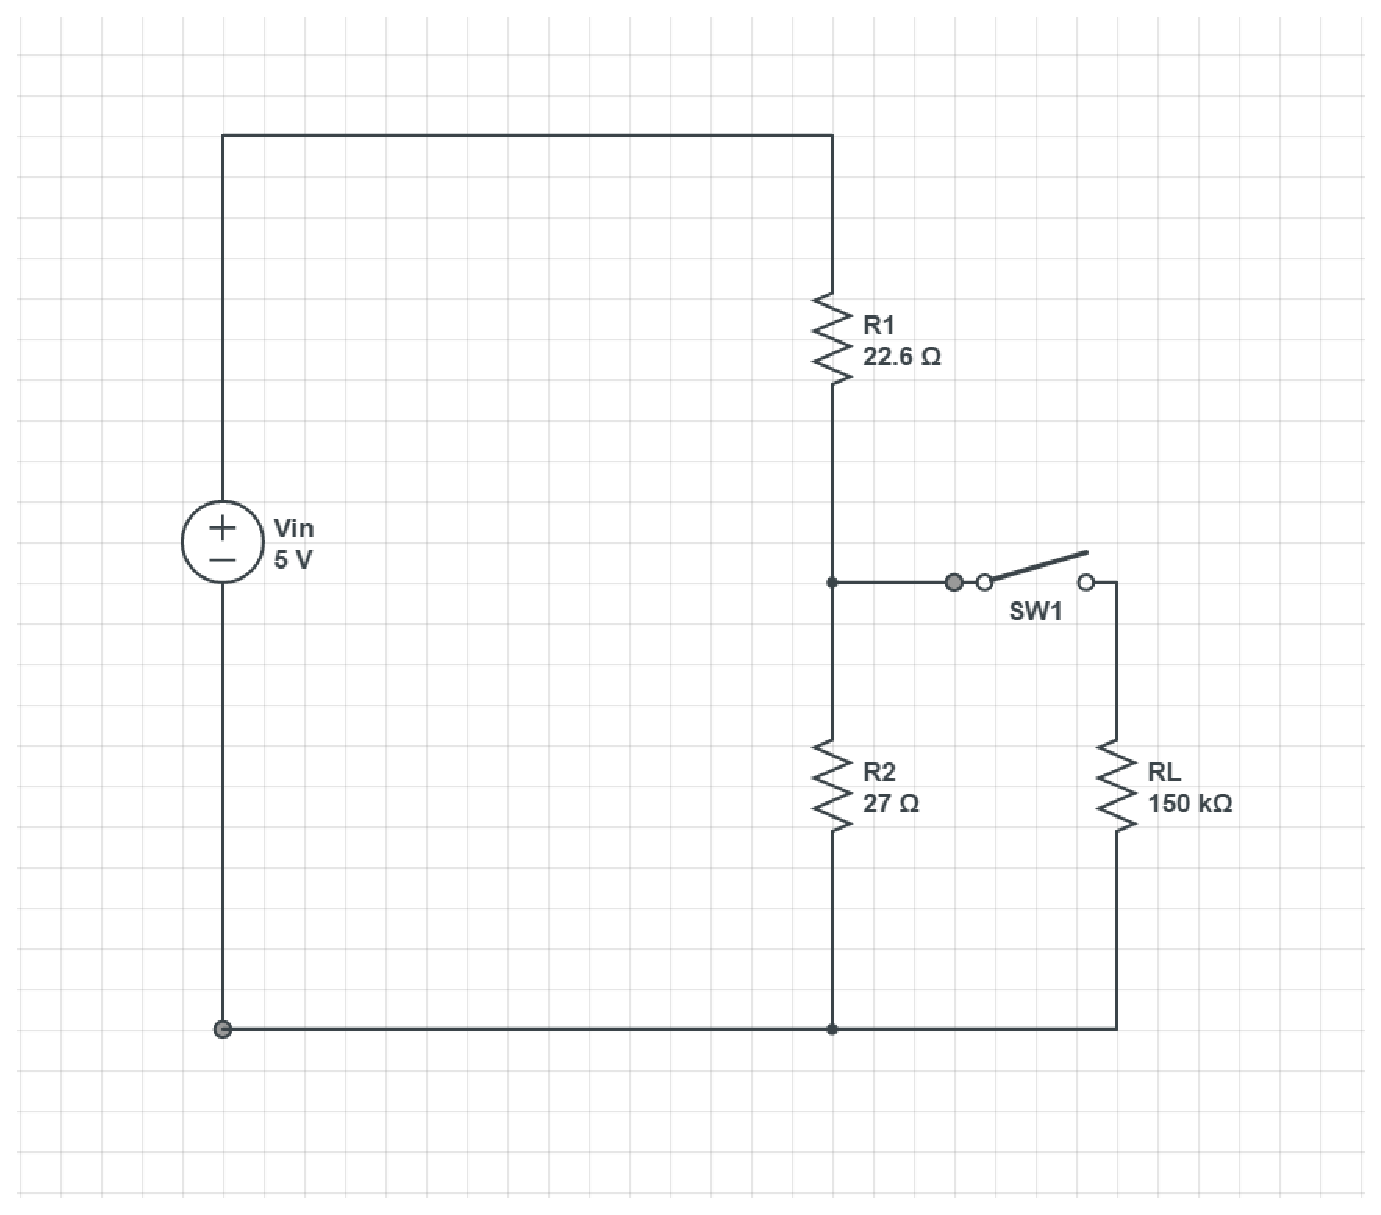
\includegraphics[scale = 0.35]{diagram2lab1.eps}  
\graphicspath{ {/home/evin/Desktop/School/Circuits/lab1/} }
\end{figure}

The circuit shown was designed to provide 2.722V to the load, $R_L$, when $R_L$ was connected and to have minimal sag. This means the voltage across $R_2$ when $R_L$ was not connected would be close to the voltage across $R_2$ when $R_L$ was connected. The measured value of the voltage across $R_L$ when connected was 2.746V. This has a 0.8817\% error from the calculated value of the output voltage which was 2.722V. Furthermore, the measured output voltage of 2.746V had a 1.704\% error from the goal of a 2.7V output. This was in part because the resistors used caused an output voltage larger than 2.7V. This was also caused by design flaws that caused the difference between the expected output voltage and the measured output voltage. Again, the resistors were not measured before added to the circuit and therefore could have had different resistances than labeled. 

The voltage across $R_2$ when $R_L$ was not connected was measured to be 2.749V. This meant that the sag was  $2.749V - 2.746V = 0.003V$. This is a very small amount of sag and achieved the goal for sag of less than 0.2V. The sag was more than it was calculated to be, but this may again be because the resistors were not measured before they were added to the circuit.


\section{Conclusion}
The goal of part A of the lab was to create a voltage divider that output 2.7V to the voltmeter. This was achieved well with only 0.4074\% error. This was close to the goal value and was within the acceptable range for the output voltage. 

For part B of the lab, the goal was to create a new voltage divider that provided 2.7V to an actual load and to minimize the sag. This part was also completed successfuly as the sag was measured to be only 0.003V and the output voltage was only 1.704\% from the desired value of 2.7V.

The error in the lab in both parts most likely came from the fact that the resistors were not tested for their resistances before being implemented into the circuit. In the future, this should be done to improve accuracy of the calculations of expected values in the circuits created.





\end{document}
